\documentclass[pdf,contemporain,slideColor,colorBG,accumulate,nototal,capsules]{prosper}
\usepackage{alltt}
\title{Open Computer Forensics Architecture API}
\author{Rob J Meijer}
\institution{Korps Landelijke Politiediensten, Driebergen, NL}
\begin{document}
\maketitle
\begin{slide}{Digital Washing Machine}
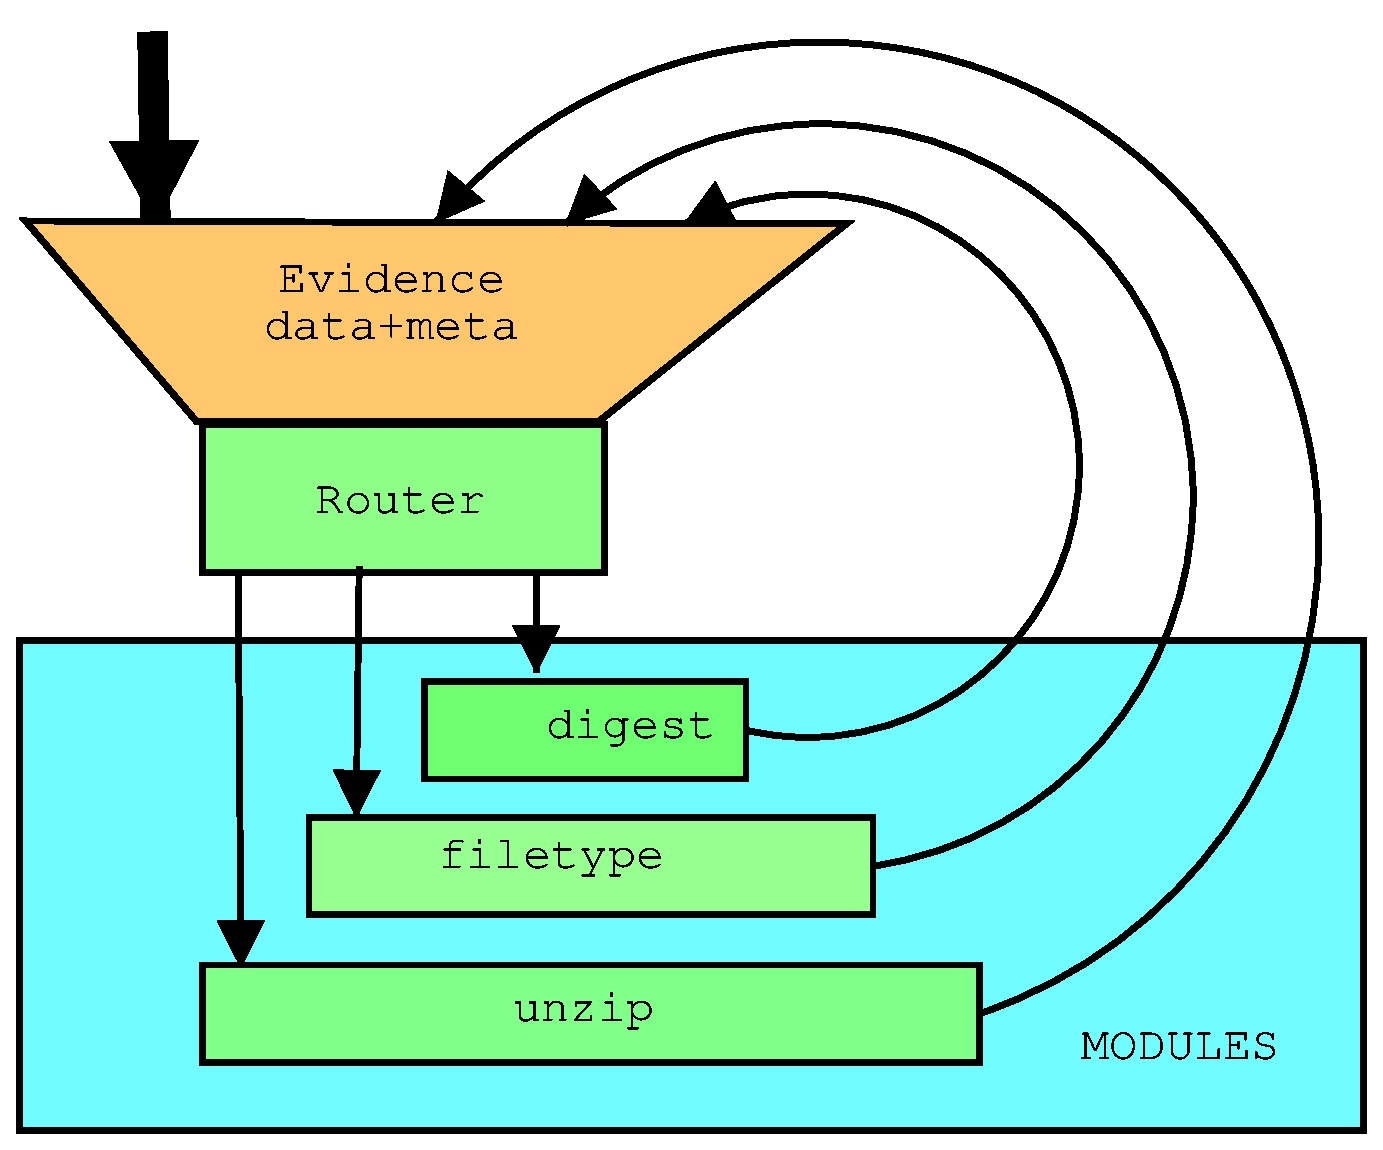
\includegraphics[width=8cm]{dia7.eps}
\end{slide}
\begin{slide}{Open Computer Forensics \\
Architecture}
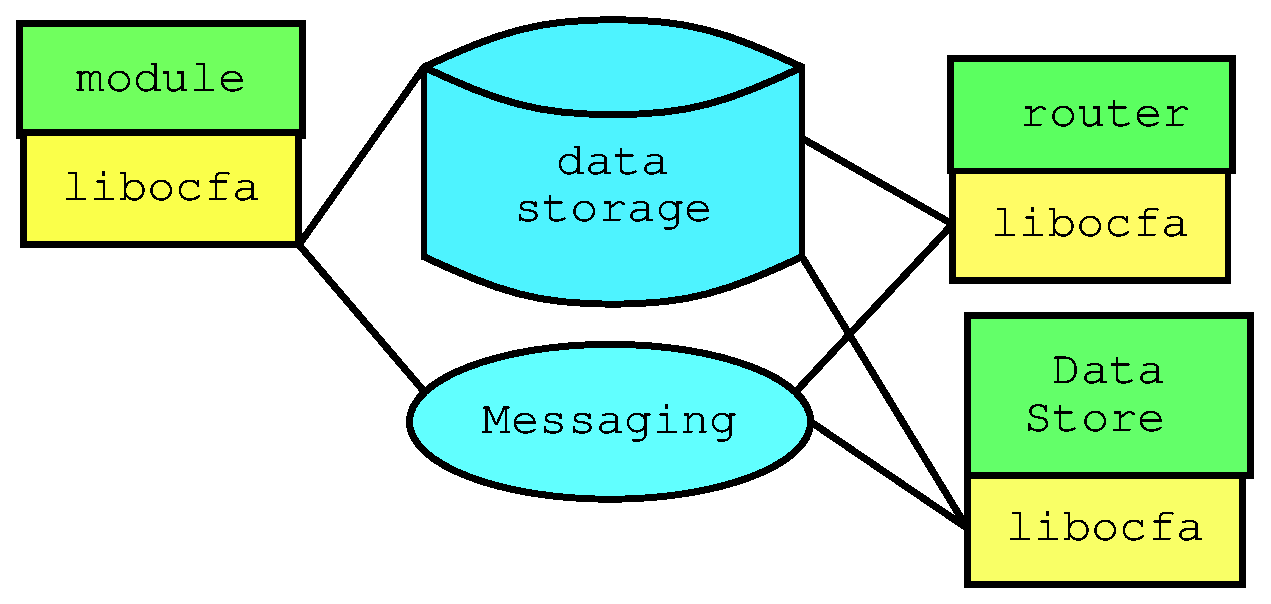
\includegraphics[width=8cm]{dia1.eps}
\end{slide}
\begin{slide}{Dual module/architecture \\
interface}
\begin{itemize}
\item OCFA Evidence API
\item Evidence XML, OCFA Message/Store API
\end{itemize}
\end{slide}
\begin{slide}{LibOcfa}
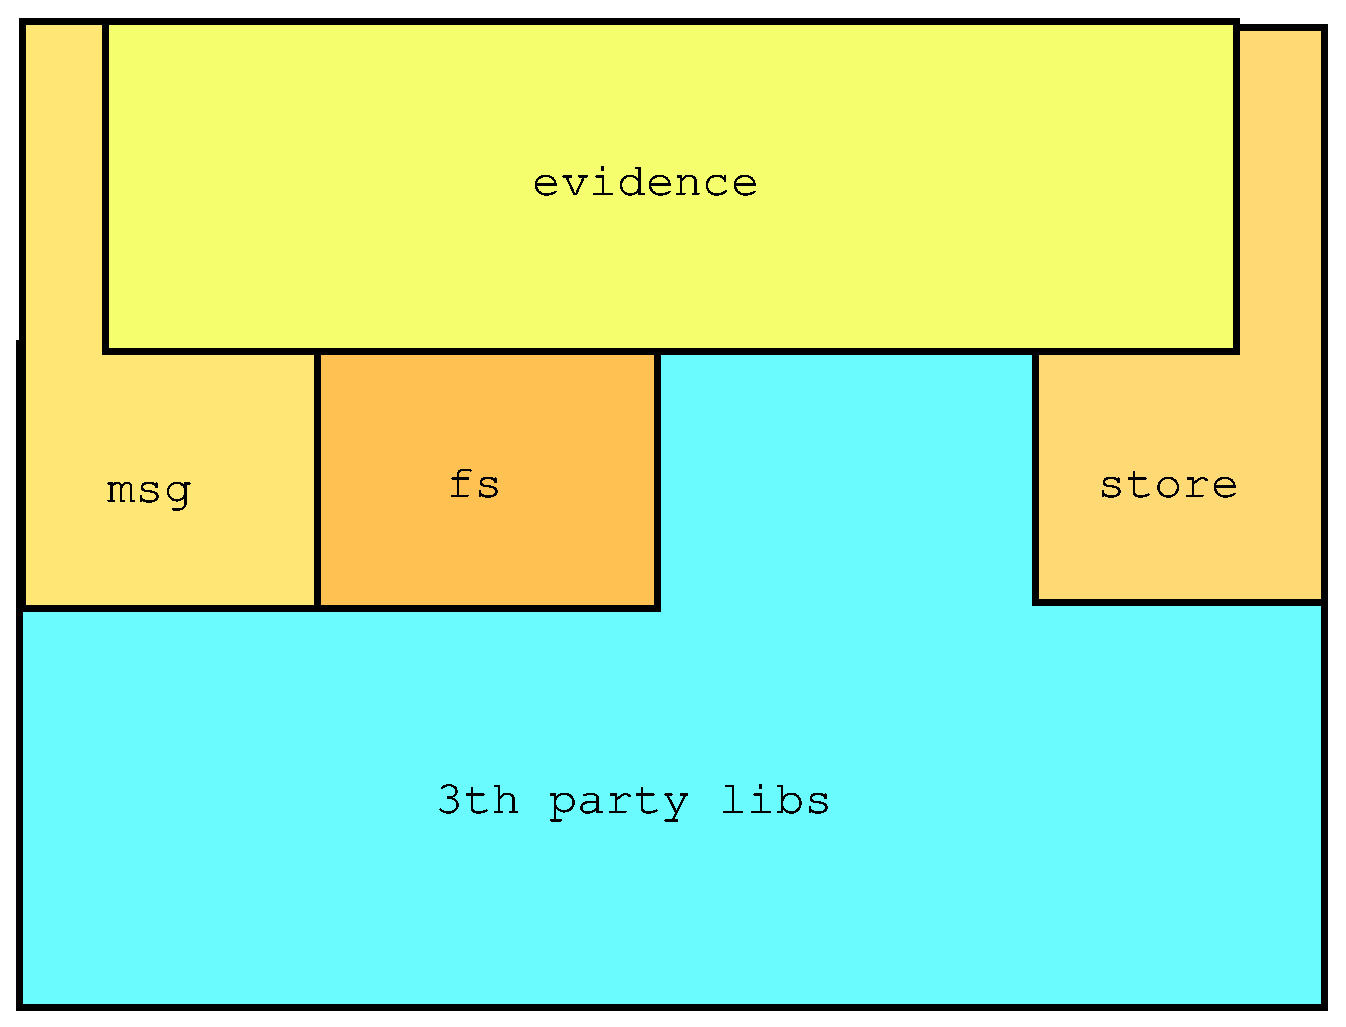
\includegraphics[width=8cm]{dia2.eps}
\end{slide}
\begin{slide}{Dependencies on 3th party libs}
  Evidence:
  \begin{itemize}
    \item libcrypto (digests)
    \item iconv (charsets)
    \item xerces (XML)
  \end{itemize}
  Store/Msg:
  \begin{itemize}
     \item libpq++ (postgress database)
  \end{itemize}
  fs/store:
  \begin{itemize}
    \item posix (libgen,unistd,stat)
  \end{itemize}
\end{slide}
\begin{slide}{XML: Evidence,Jobs \& Metadata}
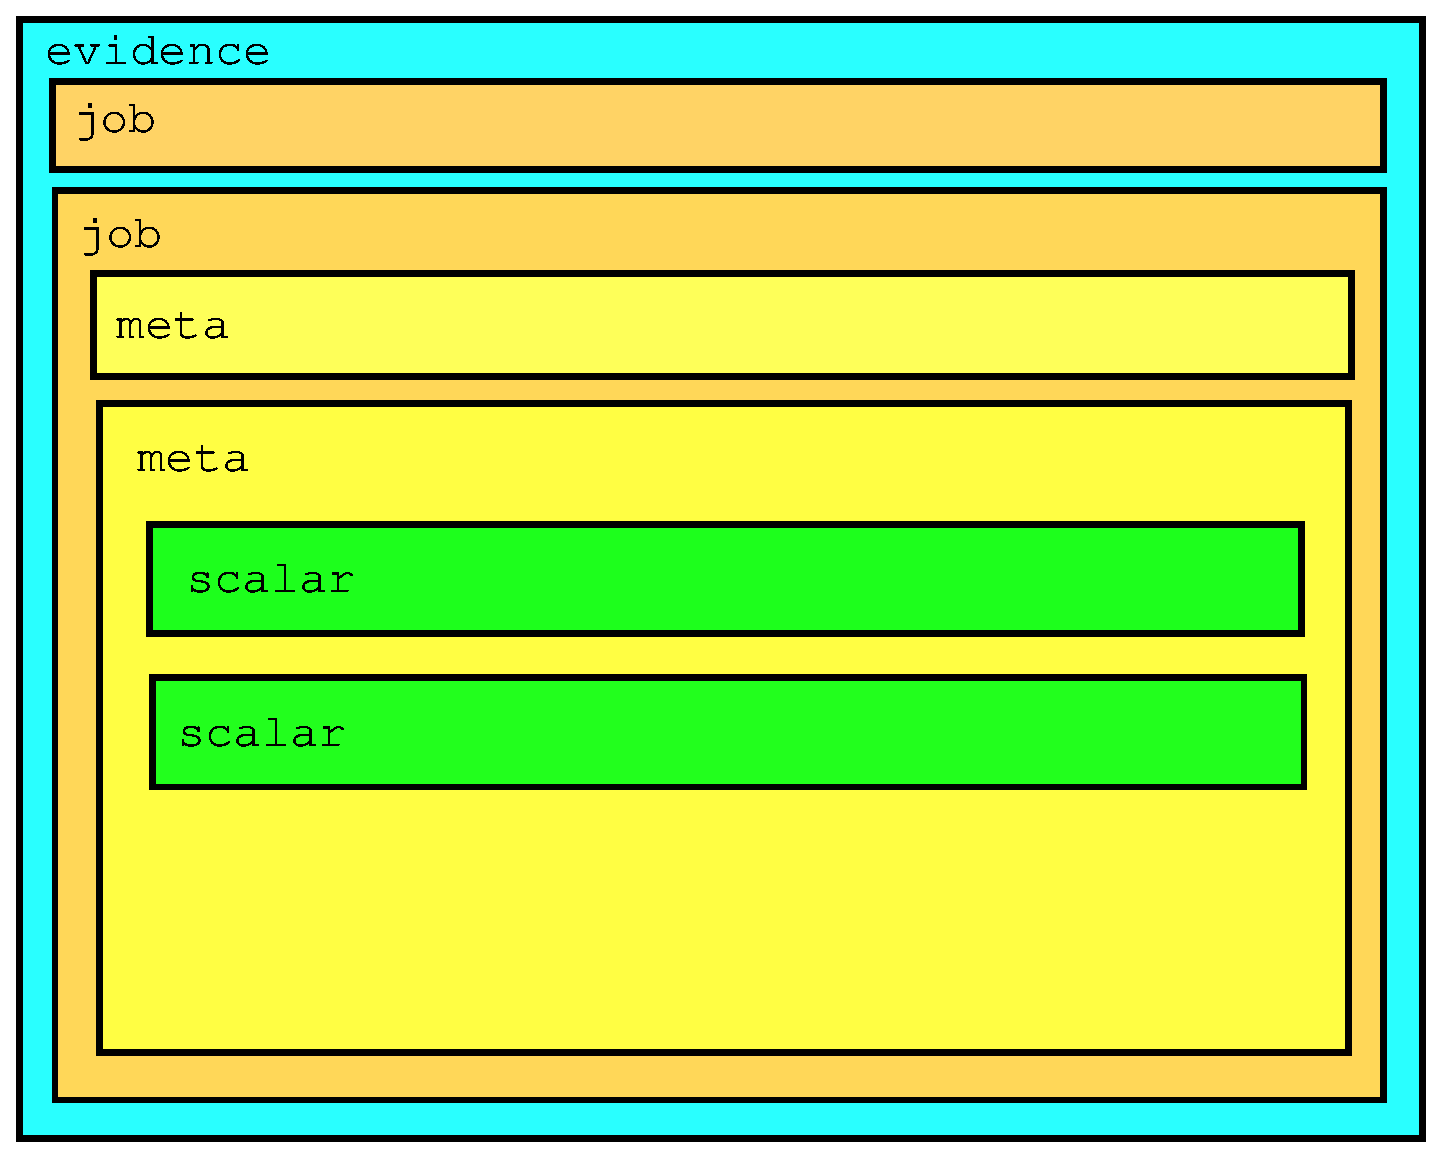
\includegraphics[width=8cm]{dia6.eps}
\end{slide}
\begin{slide}{XML : evidence}
Attributes:
  \begin{itemize}
  \item ID Fields (case,source,item,id)
  \item Digests (SHA1,MD5)
  \item status (ACTIVE / SUSPENDED / COMMITTED)
  \end{itemize}
Members:
  \begin{itemize}
  \item location
  \item job
  \end{itemize}
\end{slide}
\begin{slide}{XML : job}
Attributes
\begin{itemize}
\item timestamps (stime,etime)
\item status (NEW/PROCESSED/DONE)
\end{itemize}
Members
\begin{itemize}
\item ModuleInstance
\item Meta
\item LogLine
\end{itemize}
\end{slide}
\begin{slide}{XML: meta \& scalar}
Meta Attributes
\begin{itemize}
\item Name
\item Type (Scalar,Array,Table)
\end{itemize}
Scalar Attributes
\begin{itemize}
\item Type (Int,Float,string,datetime)
\end{itemize}
Scalar Content
\begin{itemize}
\item Int : long long
\item Float : long double
\item String : UTF8
\item datetime: unix time + sourceref
\end{itemize}
\end{slide}
\begin{slide}{Module Types}
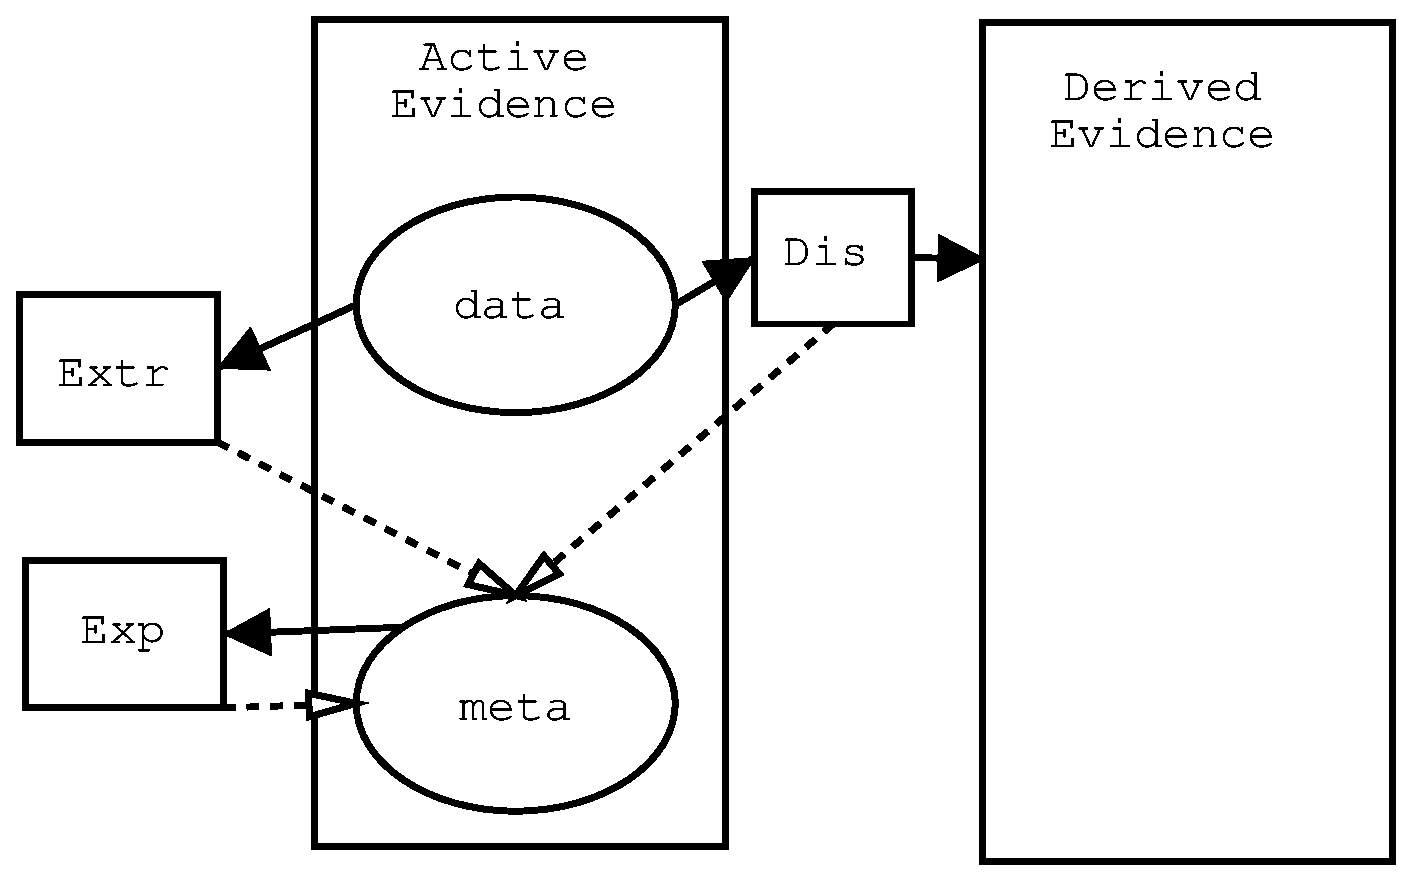
\includegraphics[width=8cm]{dia3.eps}
\end{slide}
\begin{slide}{Types \& Methods}
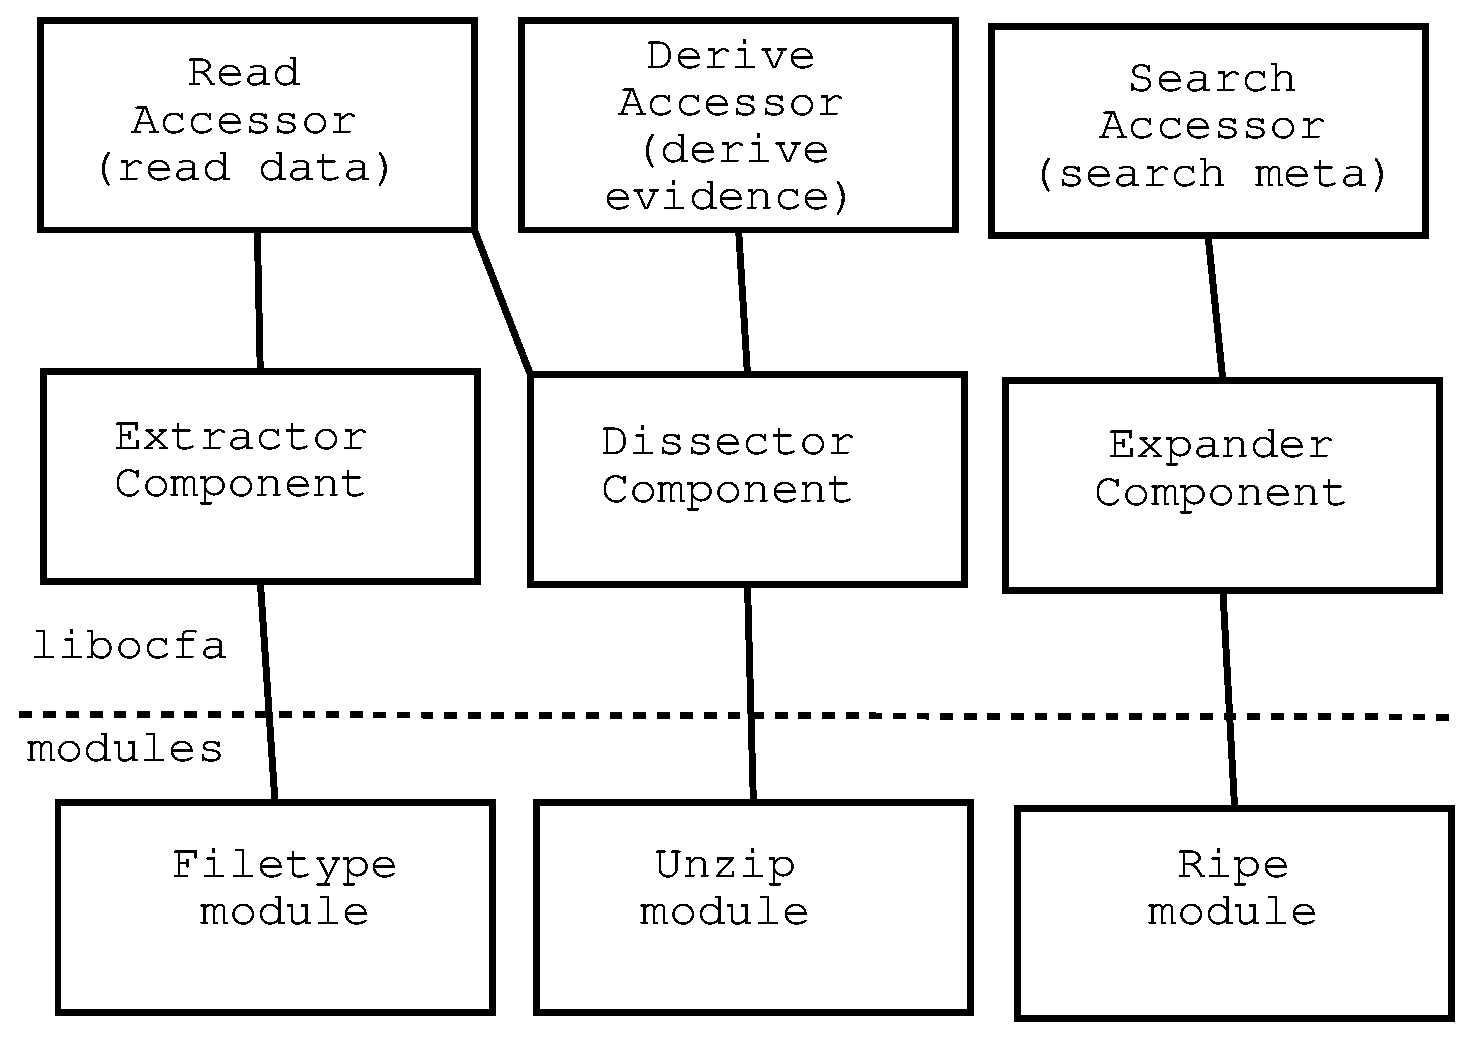
\includegraphics[width=8cm]{dia4.eps}
\end{slide}
\begin{slide}{Inheritance}
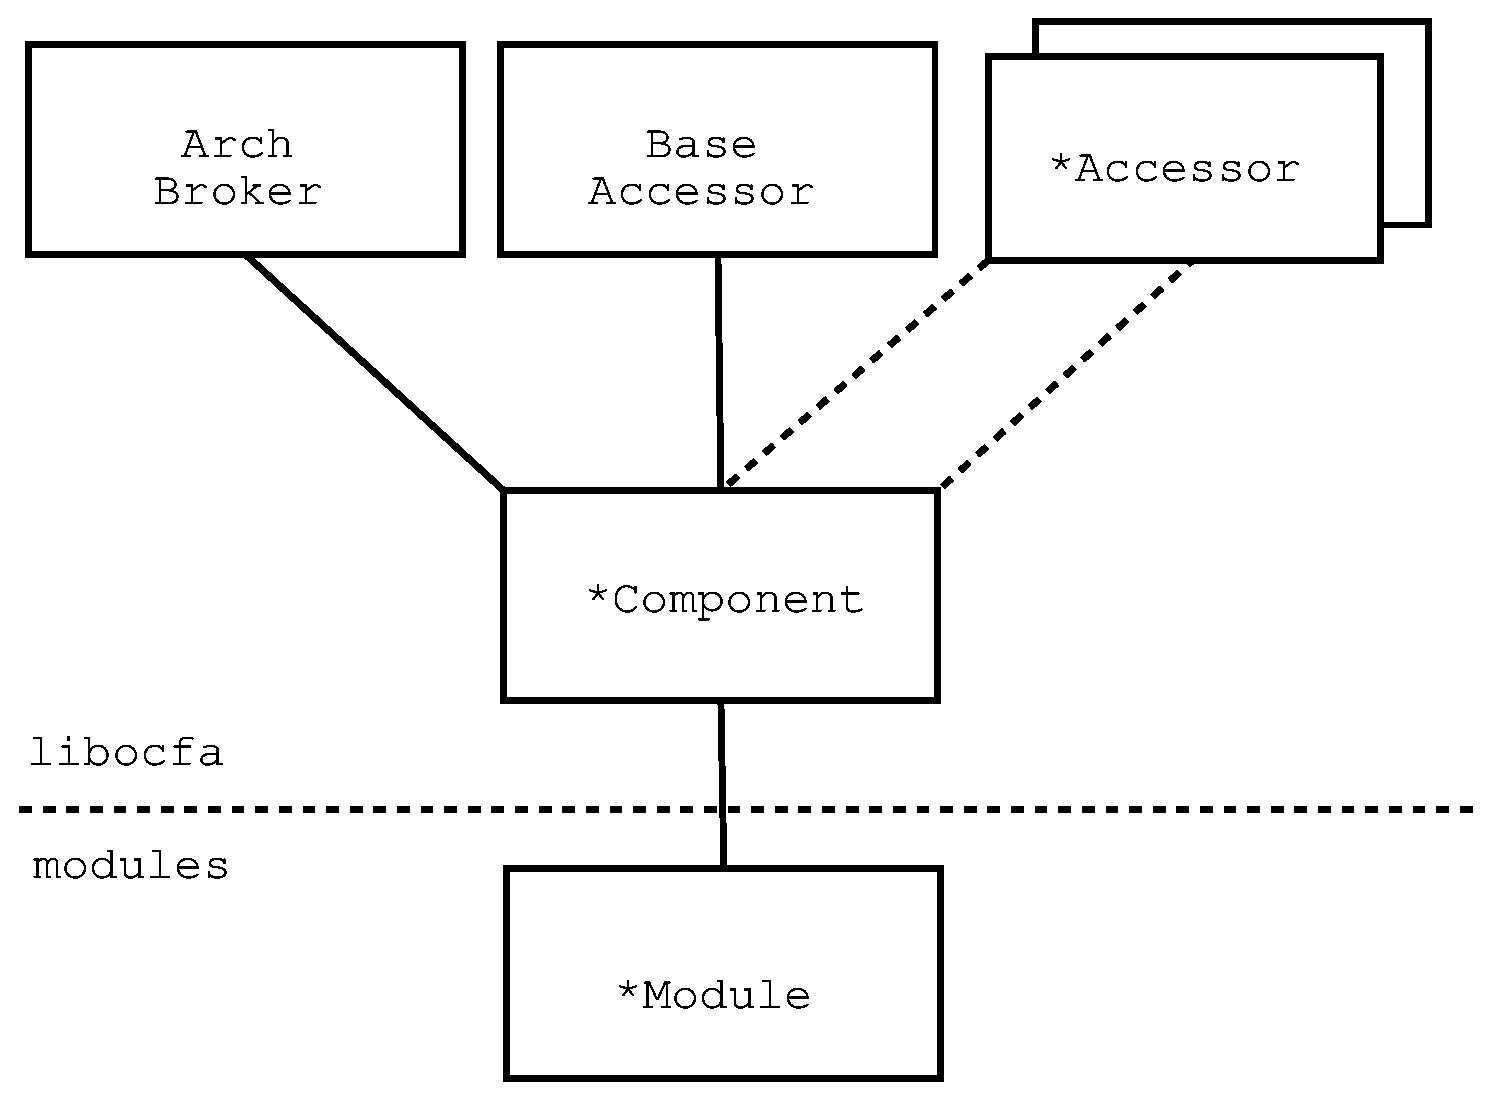
\includegraphics[width=8cm]{dia5.eps}
\end{slide}
\begin{slide}{*Accessor}
\begin{itemize}
\item  Additional 'protected' methods
\item Access to method groups of 'ActiveEvidence'
\item Access to method groups of 'ActiveJob'
\end{itemize}
\end{slide}
\begin{slide}{ArchBroker}
\begin{itemize}
\item virtual int processEvidence()
\item virtual void processMessage()
\end{itemize}
\begin{itemize}
\item void run()
\end{itemize}
\end{slide}
\begin{slide}{Module main}
\begin{alltt}
int main(int argc,char *argv[])\{
  xExtractor *x=new xExtractor();
  x->run();
\}
\end{alltt}
\end{slide}
\begin{slide}{BaseAccessor}
\begin{itemize}
\item void setMeta(name,value)
\item void pushBackMeta(name,value)
\item Scalar getEvidenceLocation()
\item string getDigestSHA1()
\item string getDigestMD5()
\end{itemize}
\end{slide}
\begin{slide}{BaseAccessor example}
\begin{alltt}
int DigestModule::processEvidence() \{
  string sha1=getDigestSHA1();
  string dsrc=somedblookupmethod(
    sha1);
  setMeta("digestsource",
    Scalar(dsrc));
  return 1;
\}
\end{alltt}
\end{slide}
\begin{slide}{ReadAccessor}
\begin{itemize}
\item EvidenceStoreEntity *getEvidenceStoreHandle()
\end{itemize}
\end{slide}
\begin{slide}{ReadAccessor example}
\begin{alltt}
EvidenceStoreEntity *estore=
  getEvidenceStoreHandle();
snprintf(cline,MAXLINE,
 "gpg -v --list-packets --batch %s",
 estore->getAsFilePath().c\_str());
command=popen(cline,"r");
\end{alltt}
\end{slide}
\begin{slide}{DeriveAccessor}
\begin{itemize}
\item string getWorkDir()
\item DerivedEvidence *derive(content,name,..)
\end{itemize}
\end{slide}
\begin{slide}{DeriveAccessor example}
\begin{alltt}
  DerivedEvidence *derived=
    derive("/output.txt",
  	   Scalar("[output]"));
  derived->setMeta("mimetype",
    Scalar("text/x-ocfa-strings"));
  derived->submit();
  delete derived;
\end{alltt}
\end{slide}
\begin{slide}{'Open' Computer Forensics \\
Architecture ??}
\begin{itemize}
\item Open API !
\item Open XML Schema !
\item Reference implementation.
\begin{itemize}
 \item Open to LEAs !
 \item Open to Vendors ?
 \item Open to the general public ?
\end{itemize}
\end{itemize}
\end{slide}
\end{document}
